\documentclass[a4paper,14pt]{extarticle}

\usepackage{cmap}
\usepackage[T2A]{fontenc}
\usepackage[utf8]{inputenc}
\usepackage[english,russian]{babel}

%\usepackage{mathptmx}% http://ctan.org/pkg/mathptmx

\usepackage{graphicx}
\usepackage{caption}
\usepackage{subcaption}
\usepackage{tabularx}
\usepackage{dcolumn}

\DeclareMathVersion{nxbold}
\SetSymbolFont{operators}{nxbold}{OT1}{cmr} {b}{n}
\SetSymbolFont{letters}  {nxbold}{OML}{cmm} {b}{it}
\SetSymbolFont{symbols}  {nxbold}{OMS}{cmsy}{b}{n}

\usepackage{geometry}

\usefont{T2A}{cmr}{m}{sl}
\linespread{1.3} % ?????????? ????????

\usepackage{indentfirst}

\usepackage[it]{titlesec}

% Table of contents styles
%\titlelabel{\thetitle\quad}
\usepackage{titletoc}

\usepackage{amsfonts}
\usepackage{mathtools}

\usepackage{hyperref}
\usepackage{url}

\def\bbljan{Jan.}
\def\bblfeb{Feb.}
\def\bblmar{Mar.}
\def\bblapr{Apr.}
\def\bblmay{May}
\def\bbljun{Jun.}
\def\bbljul{Jul.}
\def\bblaug{Aug.}
\def\bblsep{Sep.}
\def\bbloct{Oct.}
\def\bblnov{Nov.}
\def\bbldec{Dec.}


% ??????? ????? ?????????????? ??????????
\DeclareMathOperator*{\argmin}{arg\,min}

\geometry{left=35mm}
\geometry{right=20mm}
\geometry{top=20mm}
\geometry{bottom=20mm}

\titleformat*{\section}{\bfseries\filcenter}
\titleformat*{\subsection}{\bfseries\filcenter}
\titleformat*{\subsubsection}{\bfseries\filcenter}
\titleformat*{\paragraph}{\bfseries}
\titleformat*{\subparagraph}{\bfseries}

%\setcounter{secnumdepth}{0}

\usepackage{tocloft}
%\renewcommand{\cftsecleader}{\cftdotfill{\cftdotsep}}

\setlength{\parskip}{0pt}

\newcommand{\anonsection}[1]{\section*{#1}\addcontentsline{toc}{section}{#1}}

% Prevent line break in inline math
%\binoppenalty=\maxdimen
%\relpenalty=\maxdimen


\begin{document}

\begin{titlepage}
\begin{center}
  \textbf{\small
    Правительство Российской Федерации
  }
  \vspace{1.0em}
  
  \textbf{\small
    \mbox{Федеральное государственное автономное образовательное учреждение}\\
	высшего профессионального образования\\
    <<Национальный исследовательский университет \\
    <<Высшая школа экономики>>}
   \vspace{1.0em} 
    
    \textbf{\small
    \mbox{Факультет информатики, математики и компьютерных наук}\\
    Кафедра \underline{прикладной математики и информатики}
  }
\end{center}

\vspace{1.0em}

\begin{center}
  Василихин Ростислав Викторович
\end{center}

\begin{center}
  \textbf{Исследование методов определения и изменения возраста человека по фотографии}
\end{center}

\begin{center}
  Выпускная квалификационная работа по направлению\\
  \underline{Прикладная математика и информатика}\\
  магистранта группы %№
  \underline{13 МАГ ПМИ}
   (магистерская программа <<Прикладная математика и информатика>>)
\end{center}

\vspace{2.0em}

\begin{minipage}{0.5\textwidth}
  \begin{flushleft}
    Рецензент\\
    д.ф.-м.н, доцент кафедры ПМИ\\
    \underline{Н.Ю.~Золотых}
  \end{flushleft}
\end{minipage}
\begin{minipage}{0.5\textwidth}
  \begin{flushright}
    Научный руководитель\\
    преподаватель\\
    \underline{И.Д.~Лысенков}
  \end{flushright}
\end{minipage}

\vspace{\fill}
\begin{center}
Нижний Новгород, 2015
\end{center}

\end{titlepage}

\setcounter{page}{2}

\phantomsection
%\addcontentsline{toc}{section}{\contentsname}

\tableofcontents


\newpage
\anonsection{Введение}

С момента зарождения компьютерной графики одним из самых популярных объектов её исследований оставалось человеческое лицо. Как только появились методы генерации синтетических изображений, были предприняты попытки нарисовать человеческое лицо с помощью компьютера, как можно достовернее воспроизвести мимику и передать эмоции, а впоследствии --- синтезировать на компьютере реалистичные лица.

Методы <<чистой>> компьютерной графики при этом уделяют особое внимание передаче физических свойств поверхности, таких как освещённость, отражательная способность, подповерхностное рассеивание света в коже.

В то же время методы компьютерного зрения сосредоточены на анализе изображений лиц реальных людей, вычленении из них определённых наборов локальных и глобальных особенностей и комбинации их с целью получить результат, похожий на изображение из обучающей выборки. Физическим свойствам поверхности при этом уделяется второстепенное внимание.

Параметрические модели лиц, используемые в таких методах, обычно принимают в качестве параметров цвет и текстуру кожи, пропорции частей лица, описание выражения лица, словом, те параметры, которые очевидным образом задают правила для синтеза изображения. Эти параметры для реального лица возможно подобрать множеством способов, например, решая оптимизационную задачу. Однако, параметрами для синтеза изображения лица могут служить и более сложные характеристики, напрямую не связанные с внешним видом лица, такие как настроение, возраст или пол. Более того, становится возможным методами машинного обучения провести анализ и установить зависимость между <<простыми>> параметрами лица и <<сложными>>, например, можно получить классификатор, который по найденным <<простым>> параметрам лица распознаёт настроение, пол или возраст.

Отдельную задачу представляет собой определение возраста и связанная с ней задача изменения возраста по исходной фотографии. Задача определения возраста по фотографии помимо того, что является весьма сложной и интересной исследовательской задачей, имеет множество практических применений. Например, создание систем, автоматически подстраивающихся под пользователя с учётом его возраста, анализ аудитории и маркетинговые исследования, системы поиска изображений и поиска людей по изображениям. Задача изменения возраста лица по фотографии включает в себя задачу определения возраста, её решение даёт возможность состарить (или омолодить) лицо на изображении. Среди практических применений этой задачи можно выделить поиск пропавших людей (особенно детей), обновление фотографий в базах данных сотрудников, устойчивое к возрастным изменениям распознавание лиц и самое очевидное применение --- автоматическое омолаживание лица в эстетических целях.

Внешний вид лица в процессе старения зависит от многих факторов, таких как раса, пол, образ жизни, а также использование косметики, инъекций или хирургическое вмешательство. Из-за обилия этих факторов даже человек не всегда в состоянии определить возраст по фотографии достаточно точно. Создать алгоритм, способный решить такую задачу, ещё сложнее, поскольку мы сами до конца не осознаём, на какие признаки мы обращаем внимание, когда судим о возрасте, т.е. мы не знаем, как из параметров лица, которые мы можем детектировать, получить возраст. В таких случаях, когда неясно, как устроена функция от множества параметров, но известны её значения на некоторых входных данных, обычно используют машинное обучение.

Автоматическая имитация возраста предваряется анализом лиц различных возрастов и вычленением из них изменений, происходящих во время старения на разных возрастах. Для получения модифицированного изображения сначала производится предобработка исходного, затем --- автоматическое определение возраста, после чего к лицу применяются изменения, типичные для перехода от найденного возраста к целевому. 

Целью данной работы ставится анализ существующих методов автоматической оценки и автоматической имитации возраста с теоретической и практической точек зрения. Требуется изучить существующие на сегодня подходы к обеим задачам, определить, какие подзадачи необходимо для этого решить и реализовать наиболее важные из них. Поскольку задача имитации возраста включает в себя задачу определения возраста, было бы полезно рассмотреть задачу поиска возраста именно как часть системы по автоматической имитации возраста.

\newpage
\section{Автоматическое определение возраста}

\subsection{Обзор методов определения возраста}

\subsubsection{Ранние методы}
Одни из первых работ по предсказанию возраста по фото были опубликованы в девяностых годах прошлого столетия \cite{kwon1}\cite{kwon2}. Основой их медода было измерение пропорций лица, известных из антропометрических исследований, а также анализ морщин. В статье решалась задача принадлежности изображения одному из трёх кластеров: дети, молодёжь, люди среднего и пожилого возраста. Анализ пропорций позволял отделить детей от взрослых, отношение расстояния между глазами к расстоянию между глазами и носом лучше всего характеризовало принадлежность одной из этих групп. Затем для взрослых детектировались морщины, делалось это с помощью <<змеек>> (snakelets) --- сплайнов, параметры которых оптимизируются для лучшего соответствия контурам на изображении. Впрочем, эти ранние работы часто критиковались за малую тестовую выборку (47 изображений), слишком широкие возрастные группы и за необходимость больших изображений ($ 256 \times 256 $ пикселей) для детектирования морщин.

В работе \cite{horng} были развиты идеи Kwon and Lobo за счёт использования нейронных сетей для классификации по тем же признакам и расширения тестовой выборки до 230 изображений.

Анализ морщин стал популярным способом определения возраста. Так, в работе \cite{hayashi} были использованы 300 фотографий людей от 15 до 64 лет, снятые в контролируемых условиях. С помощью цветовой сегментации из изображения извлекались области с кожей лица, затем выполнялось выравнивание гистограммы (histogram equalization), чтобы выделить морщины. Для поиска морщин использовалась специальная версия алгоритма Хафа для поиска отрезков, digital template Hough transform. Алгоритм был обучен на японских лицах, и потому на всех остальных лицах выдавал низкие результаты. Отдельно было отмечена сложность поиска морщин у женщин из-за использования ими макияжа.

Авторы работы \cite{lanitis} сосредоточились на исследовании того, какие фрагменты лица позволяют лучше всего определить возраст человека. Используя созданные ими статистические модели изображения лица, они выяснили, что наилучшие результаты получаются, если для определения возраста использовать область вокруг глаз, в то же время следует исключать область лба и границу с волосами, т.к. её вариабельность лишь ухудшает результаты определения возраста. Исследователи ограничились изображениями людей до 35 лет, вследствие чего возникает сомнение, справедливы ли данные выводы для более старших возрастных групп.

\subsubsection{A Method for Automatic Synthesis of Aged Human Facial Images}
Авторы данной статьи \cite{statya_big} описали <<конвейер>> (pipeline), проходя по которому изображение претерпевает множество трансформаций, и лишь затем отдаётся на вход алгоритмам детектирования возраста. Сперва осуществляется коррекция яркости/контраста алгоритмом Retinex \cite{retinex}, затем с помощью техники, названной histogram fitting, все изображения приводятся к единому динамическому диапазону. 

\begin{figure}[t]
\centering
	\begin{subfigure}[t]{0.25\textwidth}
		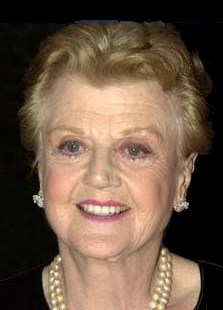
\includegraphics[width=\textwidth]{gandhi/from_57_1.png}
		\caption{оригинал}
	\end{subfigure}
	\begin{subfigure}[t]{0.25\textwidth}
		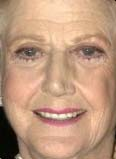
\includegraphics[width=\textwidth]{gandhi/from_57_2.png}
		\caption{искривлённое изображение}
	\end{subfigure}
	\begin{subfigure}[t]{0.25\textwidth}
		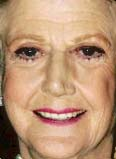
\includegraphics[width=\textwidth]{gandhi/from_57_3.png}
		\caption{с исправленной гистограммой}
	\end{subfigure}
	\caption{Коррекция изображений в методе Gandhi}
	\label{fig:gandhi}
\end{figure}

Затем оператор расставляет на изображении порядка двадцати ключевых точек, отмечая положение отдельных частей лица и на основе этих точек генерируются сплайны, подчеркивающие основные черты лица. Авторы статьи сознательно отказываются от алгоритмов автоматической разметки лица вроде ASM \cite{asm}, ссылаясь на низкое качество их работы на момент написания статьи (2004 год). После этого изображение искривляется (warp) с использованием собственного алгоритма для приведения координат отмеченных точек к координатам точек средней формы (см. рис. \ref{fig:gandhi} ).

Анализируя опыт и ошибки предшественников в автоматическом определении возраста, авторы статьи решили, что причина неудач кроется в малом количестве изображений в обучающей выборке и в низком их качестве, поэтому они собрали собственную базу изображений. Эта база состоит из 800 фотографий знаменитостей, сделанных профессиональными фотографами, отобранных вручную с целью исключить фотографии, где выражение лица далеко от нейтрального.

Для оценки возраста авторы статьи использовали метод опорных векторов, а точнее -- регрессию опорных векторов (SVR). Регрессия эта построена между числом, означающим возраст, и вектором, содержащим пиксели трансформированного изображения.

Параметры SVR, такие как вид ядра и его параметры, значение $ \varepsilon $ для чувствительности функции потерь, максимальная ошибка в критерии сходимости, были получены в результате экспериментов сперва грубо, затем с более высокой точностью с помощью кросс-валидации.

С помощью различных ухищрений, таких как переход в частотное пространство (т.е. использование в качестве входных векторов не само изображение, а его вейвлет-разложение), маскирование нелицевых областей, изменение размера изображения и т.д. удалось снизить минимальную абсолютную ошибку до 9 лет на всех возрастных группах и до 1-3 лет на отдельных образцах.

\subsubsection{Age and Gender Estimation of Unfiltered Faces}
Более современные подходы также используют модифицированный метод опорных векторов. Статья \cite{svm_dropout} вводит так называемый dropout-SVM, что позволяет им оценивать возраст изображений без ограничений по условиям съёмки. Алгоритм начинает работу с поиска лица алгоритмом Виолы-Джонса \cite{viola_jones}, затем производит выравнивание лица с использованием детектора ключевых точек, описанного в 2012 году Zhu and Ramanan \cite{zhu_ramanan}. Используя вместо самого изображения его представление с помощью локальных бинарных шаблонов \cite{lbp}, обучается обыкновенный линейный SVM-классификатор, однако интересна методика его обучения. Авторы, очевидно, были вдохновлены методом обучения искуственных нейронных сетей под названием dropout, когда в процессе обучения на отдельных итерациях временно выбрасывается какая-то доля (обычно 50\%) случайно выбранных нейронов, за счёт чего остальные нейроны лучше адаптируются к входным данным и меньше полагаются на работу соседних нейронов. А поскольку линейный SVM-классификатор реализует решающее правило, которое можно представить искуственной нейронной сетью с одним входным слоем и одним выходом, то можно провести аналогичную процедуру для входного слоя, на каждом этапе обучения случайным образом зануляя различные отдельные значения входного вектора. Полученный классификатор является гораздо более робастным (т.е. устойчивым к выбросам), чем линейный SVM, обученный традиционными методами, авторы оценивают увеличение точности минимум на 6\%.

В среднем, полученная система угадывает возрастную группу (разброс возрастов в каждой группе составляет 5-7 лет) в 67\% случаев на семейных фотографиях и почти 50\% на фотографиях из соцсетей \cite{adience}.

\subsubsection{Age and Gender Classification Using Convolutional Neural Networks}
Те же авторы буквально в мае текущего года выпустили ещё одну статью \cite{cnn_age_gender}, посвященную проблеме автоматической оценки возраста. На этот раз для оценки возраста и пола было предложено использовать свёрточные нейросети, находящиеся сегодня на очередном пике популярности. Архитектура нейросети, предложенная авторами, позволяет передать на вход отмасштабированное до $256 \times 256$ RGB-изображение лица, в произвольной позе и с произвольным выражением лица, и получить на выходе одну из возрастных категорий:
\begin{itemize}
\item от 0 до 2 лет
\item от 4 до 6 лет
\item от 8 до 12 лет
\item от 15 до 20 лет
\item от 25 до 32 лет
\item от 38 до 43 лет
\item от 48 до 53 лет
\item от 60 до 100 лет
\end{itemize}

Нейросеть состоит из трёх свёрточных слоёв (96 фильтров $7 \times 7$, 256 фильтров $5 \times 5$, 384 фильтров $3 \times 3$) и двух полносвязных, каждый по 512 нейронов (см. рис. \ref{fig:cnn}). На всех слоях в качестве активационной функции используется ReLU, один из вариантов которой выглядит так:

$$
f(x)={\begin{cases}x,&{\mbox{if }}x>0\\0.01x,&{\mbox{otherwise}}\end{cases}}
$$

Использование ReLU - довольно популярная практика в обучении нейросетей. Смысл использования ReLU состоит в добавлении нелинейности, что, по некоторым данным, даёт возможность приблизить с помощью нейросети практически любую функцию. Другим важным свойством ReLU является то, что её градиент либо равен единице, либо очень близок к нулю, и, следовательно, не может произойти разрастание или затухание градиентов при обучении нейросети методом обратного распространения ошибки.

\begin{figure}[t]
	\centering
	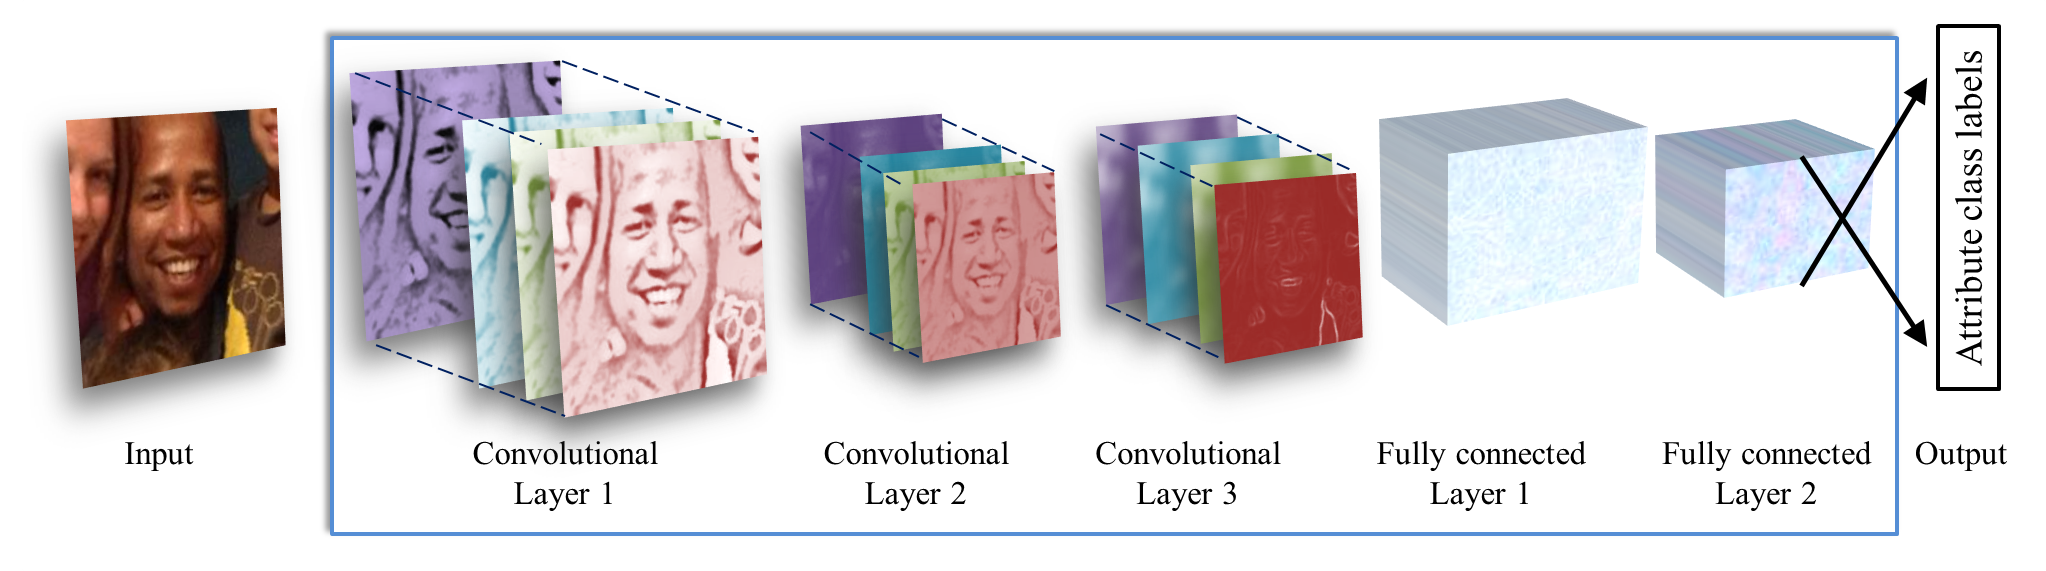
\includegraphics[width=\textwidth]{cnn.png}
	\caption{Архитектура нейросети для определения возраста}
	\label{fig:cnn}
\end{figure}

Авторы отмечают, что относительно малое число слоёв было использовано с целью избавиться от переобучения, столь характерного для других популярных алгоритмов определения возраста. Что интересно, авторы используют такую же архитектуру нейронных сетей для определения пола, но в качестве выходного слоя используется всего два выхода.

К достоинствам описанного подхода можно отнести простоту реализации. Для определения возрастной группы человека достаточно простейшей предобработки изображения (кадрирование лица и масштабирование до размера, принимаемого нейросетью), после этого для оценки возраста достаточно будет воспользоваться обученными весами нейросети и произвести один прямой проход по сети, что можно сделать с помощью любого фреймворка для работы с нейросетями.

Недостатки у этого подхода в целом такие же, как и у всех методов, использующих нейросети, однако, связаны они не с качеством работы метода, а с недостаточно проработанной теорией нейросетей. Так, выбор архитектуры сети ничем не обусловлен; метод в явном виде не производит нормализацию изображения, поиск ключевых точек и остальные необходимые операции из <<конвееров>> по оценке возраста. Исследователи полностью полагаются на нейросеть, в надежде, что все эти операции в неявном виде будут реализованы на различных её уровнях. Это означает, что если на некоторых наборах входных данных результаты будут неудовлетворительными, останется лишь гадать, почему. Кроме того, исследователи не учитывают процесс старения лица вообще, в частности, определение возраста происходит по неупорядоченным группам. Поэтому они, однако, с такой лёгкостью адаптировали нейросеть всего к двум кластерам для определения пола, исходя, видимо, из соображения, что внешность людей разных возрастов с точки зрения компьютера отличается так же сильно, как и внешность людей разных полов.

Однако, цель работы - рассмотреть наиболее предпочтительные подходы с практической, а не с теоретической точки зрения. И если производительность этого подхода окажется выше, чем у конкурирующих, это достоинство перевесит все перечисленные недостатки.

\subsection{Эксперименты с оценкой возраста}

Для оценки производительности был выбран последний из описанных методов, использующий искусственные нейросети. Главной причиной тому является то, что авторы выложили обученную ими нейросеть, что даёт нам возможность не задумываться о неочевидных деталях, которые мы могли бы упустить при самостоятельной реализации метода, а сосредоточиться на практической проверке его качества. Что касается остальных методов оценки возраста, то методы 2004 года и ранее предъявляют очень высокие требования к качеству входных изображений и сопутствующих данных. Так, метод из статьи Gandhi \cite{statya_big} обязательно требует изображений в хорошем разрешении, снятых в закрытом помещении с равномерным светом, не говоря уже о том, что он требует от пользователя вручную расставить на изображении ключевые точки. Несмотря на то, что с 2004 года появилось несколько детекторов ключевых точек с гораздо более высокой точностью, чем популярные в то время, такие как детекторы от Jason Saragih \cite{jsaragih} или от Zhu и Ramanan \cite{zhu_ramanan}, требование расставлять точки вручную означает практически абсолютную точность, без которой корректная работа алгоритма не может быть гарантирована. Авторы же подхода с использованием нейросетей заявляют, что их метод устойчив к плохим условиям съёмки.

Для оценки производительности данного метода был использован набор изображений Adience Benchmark \cite{adience}. Изображения в данном датасете были собраны из социальной сети Flickr и снабжены подробными описаниями, включающими в себя индивидуальный номер, закреплённый за каждым человеком с фотографий, пол, возрастную группу (с разбросом в 5-7 лет), а также некоторые данные о геометрии лица, включая описывающй лицо прямоугольник и оценённые автоматически углы поворота головы в трёхмерном пространстве. Пользуясь этой информацией, изображения были подвергнуты афинным преобразованиям с целью выровнять лица до пропорций, близких к пропорциям лиц анфас. База данных содержит порядка 20000 изображений, снятых преимущественно любителями на камеры смартфонов, в базе большое количество совместных фотографий, сэлфи, фотографий с посторонними объектами, с низкой четкостью и неровным освещением.

Такой набор данных позволит выяснить, насколько алгоритм устойчив к помехам, искажениям и плохим условиям съёмки. Более того, можно будет выяснить, насколько сильно зависит результат работы алгоритма от условий съёмки, отобрав фотографии с различным качеством и проследив за тем, возникают ли ошибки определения возраста чаще на низкокачественных фотографиях.

Из всех изображений базы были случайно выбраны 3210 изображений. Из базы были исключены изображения, для которых не указан возраст или указанный возраст находится вне возрастных рамок, которые способен был бы определить алгоритм. Остальные изображения были пропущены через обученную авторами работы нейросеть, после чего было проведено сравнение реального возраста с оценённым. Для тестирования был использован фреймворк для работы с искусственными нейросетями Caffe и Numpy для загрузки изображений и их подготовке для нейросети.

Оценка качества алгоритма производилась с учётом того, что он на самом деле решает не задачу регрессии между возрастом и характеристиками изображения, а задачу классификации изображения как принадлежащего одному из классов. Поэтому было оценено не только число лет, на которое ошибся алгоритм, но и ошибка в определении возрастной группы. Во внимание были также приняты результаты, полученные авторами статьи.

Результаты приведены в таблице \ref{table:age_precision}. Они в среднем на 3\% ниже, чем результаты, приведённые авторами статьи, что можно объяснить меньшей выборкой для тестирования.

\newcolumntype{d}[1]{D{,}{,}{#1} }
\makeatletter
\newcolumntype{B}[3]{>{\boldmath\DC@{#1}{#2}{#3} }c<{\DC@end} }
\newcolumntype{Z}[3]{>{\mathversion{nxbold}\DC@{#1}{#2}{#3} }c<{\DC@end} }
\makeatother

\begin{table}
\caption{Точность детектирования возраста}
\small
{
\begin{tabular}{|l|d{2}|d{2}|d{2}|d{2}|r|}
\hline
Возраст & 
\multicolumn{1}{c|}{ \parbox[t]{2.35cm}{ верно \\ угаданных, \%} }  & 
\multicolumn{1}{c|}{ \parbox[t]{2.35cm}{ Средняя \\ ошибка, лет } } & 
\multicolumn{1}{c|}{ \parbox[t]{2.35cm}{ Средняя \\ абсолютная \\ ошибка, лет } } &
\multicolumn{1}{c|}{ \parbox[t]{2.35cm}{ Стандартное \\ отклонение, лет } } & 
\parbox[t]{2cm}{ Общее \\ кол-во } \\
\hline
\enspace 0 - 2   & 65,03 &   2,77 &  2,77 &  6,32 &  675 \\
\enspace 4 - 6   & 33,97 &   2,70 &  5,26 &  8,93 &  365 \\
\enspace 8 - 12  & 60,00 &   4,54 &  6,76 & 12,03 &  160 \\
        15 - 20  &  0,00 &   8,69 & 12,39 & 10,88 &  111 \\ 
        25 - 32  & 58,96 &  -4,04 &  7,74 & 12,08 & 1143 \\
        38 - 43  & 20,29 & -14,36 & 14,55 & 12,19 &  404 \\
        48 - 53  &  0,02 & -23,74 & 23,74 & 13,55 &  167 \\
        60 - 100 &  0,06 & -45,70 & 45,70 & 18,08 &   94 \\
\hline
Всего &  45,69 &  -4,39 &  9,37 & 14,72 & 3121 \\
\hline
\end{tabular}
}
\label{table:age_precision}
\end{table}

В первую очередь нужно заметить, что несмотря на результат в 45\% угадывания возрастной категории, средняя ошибка в определении возраста составляет чуть более девяти лет, как и в старом алгоритме из статьи Gandhi \cite{statya_big}. Кроме того, возможно, набор обучающих изображений для нейросети не был сбалансирован, поскольку лишь на двух категориях изображений достигается результат около 60\% и выше (от 0 до 2 лет и от 25 до 32 лет), за счёт них нейросеть и имеет такой относительно высокий средний результат детектирования.

\begin{table}
\caption{Результаты классификации возраста, \%}
\normalsize 
{
\begin{tabular}{|l|d{1} d{1} d{1} d{1} d{1} d{1} d{1} d{1}|d{1}|}
\hline
Возраст &
\multicolumn{1}{c}{0-2}   &
\multicolumn{1}{c}{4-6}   &
\multicolumn{1}{c}{8-12}  &
\multicolumn{1}{c}{15-20} &
\multicolumn{1}{c}{25-32} &
\multicolumn{1}{c}{38-43} &
\multicolumn{1}{c}{48-53} &
\multicolumn{1}{c|}{60-100}&
\multicolumn{1}{c|}{Доля} \\
\hline
\enspace 0 - 2   & \multicolumn{1}{Z{,}{,}{1}}{65,0} & 23,9 &  7,4  &  0,0 &    2,8 &  0,6 &   0,3 &  0,0 & 21,6 \\
\hline
\enspace 4 - 6   & 32,0 & \multicolumn{1}{Z{,}{,}{1}}{33,9} & 23,2  &  0,0 &    9,0 &  1,6 &   0,3 &  0,0 & 11,7 \\
\hline
\enspace 8 - 12  &  6,8 &    9,9 & \multicolumn{1}{Z{,}{,}{1}}{59,6}&  0,0 &   14,9 &  8,1 &   0,0 &  0,6 &  5,2 \\
\hline
        15 - 20  &  4,5 &    1,8 & 11,7 & \multicolumn{1}{Z{,}{,}{1}}{0,0} &   73,0 &  7,2 &   0,9 &  0,9 &  3,6 \\
\hline
        25 - 32  &  8,0 &    3,9 & 14,9 &  0,3  & \multicolumn{1}{Z{,}{,}{1}}{59,0} & 13,0 &   0,7 &  0,3 & 36,6 \\
\hline
        38 - 43  &  9,7 &    2,2 &  9,9 &  0,2  & 56,4 & \multicolumn{1}{Z{,}{,}{1}}{20,5} &   1,0 &  0,0 & 12,9 \\
\hline
        48 - 53  & 13,8 &    2,4 &  5,4 &  0,0  & 50,9 &   24,6 & \multicolumn{1}{Z{,}{,}{1}}{3,0} &  0,0 &  5,4 \\
\hline
        60 - 100 &  8,5 &    2,1 &  6,4 &  0,0  & 26,6 &   44,7 &  5,3 & \multicolumn{1}{Z{,}{,}{1}|}{6,4} &  3,0 \\
\hline
 ~~     Все      & 18,5 &   10,0 & 17,3 &  0,1  & 36,6 &   15,0 &  1,4 &   1,0 & 100,0 \\
\hline
\end{tabular}
}
\label{table:age_confusion}
\end{table}

В таблице \ref{table:age_confusion} представлено распределение результатов классификации внутри каждого кластера: для каждого фиксированного реального возраста в строке указана условная вероятность детектирования каждого кластера из столбца.


На всех группах изображений дисперсия ошибки больше, чем разброс внутри группы, что говорит о том, что б$ \grave{o} $льшая часть ошибок в детектировании пришлась на соседние группы. Действительно, реальная возрастная группа отличается от предсказанной не более чем на один соседний кластер в 75\% случаев. Эти результаты подтверждаются авторами статьи, которые пишут о 80\% угадывании с ошибкой в один кластер.

Анализ ошибочных изображений подтвердил некоторые выводы, сделанные ранее. Так, если на изображении - женщина, это увеличивает вероятность ошибки, причём в отрицательную сторону. Отчасти это связано с использованием макияжа. Однако более вероятно, что дело здесь в том, что нейросеть обучалась одновременно и на мужчинах, и на женщинах. Процесс старения же у мужчин и женщин отличается, как правило мужские лица с возрастом меняются значительно быстрее. В результате лица с меньшими возрастными изменениями воспринимаются нейросетью как более молодые.

А вот нетребовательность алгоритма к условиям съёмки была подтверждена. В процессе анализа ошибочных изображений не было выявлено зависимости между качеством фотоснимка и размером ошибки. Среди верно классифицированных изображений присутствовали как изображения в хорошем качестве с ровным освещением, так и низкокачественные фотографии с размытыми деталями, неровным светом и экстремальными выражениями лица.


\newpage
\section{Автоматическая имитация возраста}

Методы имитации возраста подразделяются на две категории. Методы первой категории используют знания, полученные из анатомических исследований кожи и мимики лица, чтобы затем интерпретировать определенные параметры лица как критерии возраста. Методы второй категории используют алгоритмы машинного обучения для того, чтобы автоматически вычленить те изменения в параметрах лица, что соответствуют старению. 

\subsection{Методы, основанные на анатомии лица}

Измеряя такие параметры лица, как высота лба, размер носа, положение уголков губ у женщин от 25 до 65 Pitanguy et al. \cite{pitanguy1} \cite{pitanguy2} установили строгую корреляцию между этими параметрами и возрастом. В результате была построена модель имитации возраста, основанная на изменении пропорций и искривлении (warping) изображения. Впоследствии были применены методы из трехмерной графики для получения результатов, достаточно хороших, по мнению авторов, для прогнозирования операций в пластической хирургии.

Hussein \cite{hussein} предложил измерять на нейтральных лицах геометрические изменения лица, а также изменения в текстуре путём сравнения их BRDF (двулучевых функций отражательной способности), определяющих, как поверхность поглощает и отражает свет.

В целом, анализ подобных методов свидетельствует \cite{statya_big}, что наиболее заметные изменения лица с возрастом происходят не с геометрическими характеристиками, а с текстурой: появляются морщины, пятна, щетина. Из-за этого методы, основанные на антропометрии, показывают не очень реалистичные результаты, так как им не удаётся контролировать все параметры, формирующие внешний вид человеческого лица.

\subsection{Методы, основанные на статистических моделях}

\subsubsection{Некоторые ранние методы}
В ранее упоминавшейся работе Lanitis \cite{lanitis} использовалась статистическая модель, основанная на активной модели формы (ASM) Кутеса и Тейлора, 1995 \cite{asm}. Модель подразделяется на модель формы (в точности заимствованная из оригинального метода ASM \cite{asm}, использующая метод главных компонент для вектора координат ключевых точек) и модель текстуры из 3600 черно-белых пикселей, где также используется метод главных компонент для описания текстуры лица в нейтральном положении. Таким образом, пренебрегая выражением, текстуру каждого лица можно было описать вектором коэффициентов перед собственными векторами (использовалось порядка 50 собственных векторов). Далее авторы подобрали квадратичную функцию от этих коэффициентов, как можно более точно приближающую возраст человека.

Для синтеза лица с другим возрастом требуется подобрать обратную функцию, которая для заданного возраста выдавала бы набор коэффициентов для текстуры лица. Авторы решили эту задачу, сгенерировав большое количество векторов коэффициентов, оценив для них возраст и сопоставив каждому возрасту наиболее популярные наборы коэффициентов. Подбор коэффициентов именно под конкретное лицо осуществляется из соображений о том, как меняются векторы коэффициентов с возрастом и по похожести лица на примеры из базы, для которых эти зависимости рассчитаны.

\begin{figure}[t]
\centering
	\begin{subfigure}[t]{0.2\textwidth}
		
\includegraphics[width=\textwidth]{gandhi/lanitis1.png}
		\caption{оригинал}
	\end{subfigure}
	\begin{subfigure}[t]{0.2\textwidth}
		
\includegraphics[width=\textwidth]{gandhi/lanitis2.png}
		\caption{имитация возраста}
	\end{subfigure}
	\begin{subfigure}[t]{0.2\textwidth}
		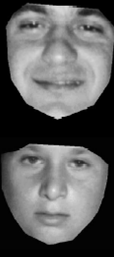
\includegraphics[width=\textwidth]{gandhi/lanitis3.png}
		\caption{реальное лицо}
	\end{subfigure}
	\caption{Результаты из работ Lanitis et al. \cite{lanitis2}}
	\label{fig:lanitis}
\end{figure}

При этом в работах  Lanitis et al. \cite{lanitis} \cite{lanitis2} \cite{lanitis3} для обучения были взяты изображения различного качества с различным освещением, выражением лица, поворотом головы и т.д. Результаты приведены на рис. \ref{fig:lanitis}.

Shan et al. \cite{shan} предложили метод под названием Image-Based Surface Detail Transfer (IBSDT), суть которого в переносе с одного изображения на другое мелких деталей вроде морщин и родинок или больших деталей, таких, как скулы или форма крыльев носа. К сожалению, метод не полностью автоматический, выбор изображения, с которого следует брать детали, должен совершать оператор.

\begin{figure}[t]
	\centering
	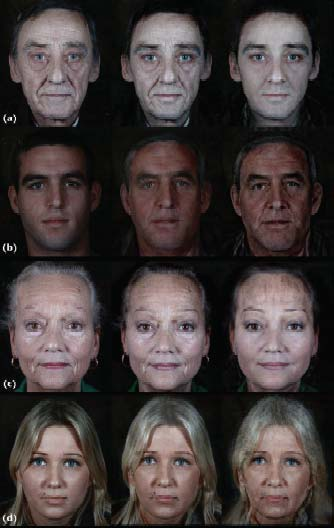
\includegraphics[width=0.3\textwidth]{gandhi/tiddeman.png}
	\caption{Результаты из работы Tiddeman et al. \cite{tiddeman}}
	\label{fig:tiddeman}
\end{figure}

Tiddeman et al. \cite{tiddeman} использовали вейвлеты для описания и преобразования текстуры лица. Имея для каждой возрастной группы лицо-прототип, авторы оценили направления изменений между прототипами для таких не-визуальных параметров, как возраст, пол или раса. Эти изменения затем применялись ко входному лицу. Чтобы результирующее изображение не было слишком гладким (как это бывает во многих методах имитации возраста), прототипы подстраивались под границы, детектируемые на изображении с помощью вейвлетов Габора, основанных на принципах восприятия изображения человеческим глазом (см. рис. \ref{fig:tiddeman}).


\subsubsection{A Method for Automatic Synthesis of Aged Human Facial Images}
Авторы уже упоминавшейся статьи Gandhi \cite{statya_big} описали <<конвейер>> (pipeline), проходя по которому изображение претерпевает множество трансформаций, и лишь затем отдаётся на вход алгоритмам детектирования возраста.

Для имитации изменений возраста авторы предложили воспользоваться методом IBSDT, описанном в статье Shan et al. \cite{shan}. Идея состоит в том, что если наивно перенести изменения между изображениями лиц разных возрастов на новое лицо, то оно будет выглядеть старше (или моложе, в зависимости от того, как считать разницу между изображениями). Например, если на молодое лицо наложить морщины, оно будет выглядеть старше. При этом считается, что лица имеют одинаковые выражения и одинаковое положение всех частей лица. Однако, такая модификация лица не учитывает различный цвет кожи во входном изображении и в обучающих изображениях.

IBSDT исходит из предположения, что изображения лиц соответствуют ламбертовой модели отражения света:
$$
I(P) = \rho(P) l \left \langle \mathbf{n}(P), \mathbf{l}(P) \right \rangle
$$

\begin{figure}[t]
\centering
	\begin{subfigure}[t]{0.2\textwidth}
		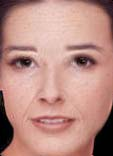
\includegraphics[width=\textwidth]{gandhi/sim1.png}
		\caption{$\sigma = 1$ }
	\end{subfigure}
	\begin{subfigure}[t]{0.2\textwidth}
		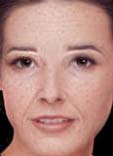
\includegraphics[width=\textwidth]{gandhi/sim2.png}
		\caption{$\sigma = 2$ }
	\end{subfigure}
	\begin{subfigure}[t]{0.2\textwidth}
		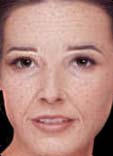
\includegraphics[width=\textwidth]{gandhi/sim3.png}
		\caption{$\sigma = 3$ }
	\end{subfigure}
	\begin{subfigure}[t]{0.2\textwidth}
		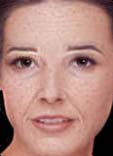
\includegraphics[width=\textwidth]{gandhi/sim4.png}
		\caption{$\sigma = 4$ }
	\end{subfigure}
	\caption{Имитация старения с различными значениями $\sigma$}
	\label{fig:sigmas}
\end{figure}

IBSDT решает проблему переноса нормалей с одного изображения на другое. Из допущения о константности альбедо выводится следующее преобразование изображения:

$$
\widehat{I}_2 = \frac {I_1} {\overline{I}_1} \overline{I}_2
$$

где $ I_1 $ --- изображение, откуда требуется взять нормали, $ I_2 $ --- исходное изображение, на которое требуется перенести нормали, $ \overline{I} $ --- изображение, размытое фильтром Гаусса с некоторым значением параметра $\sigma$ (см. рис. \ref{fig:sigmas}).

Изображения-прототипы были рассчитаны для возрастных групп с разбросом возрастов в 5 лет. Вместо усреднения изображений в группе, которое, по мнению авторов, скрадывает морщины и другие значительные для <<состаривания>> детали, было решено использовать последовательное применение IBSDT к среднему по группе:

$$
\widehat{I} = \frac {I_1} {\overline{I}_1} \cdot \frac {I_2} {\overline{I}_2}  \cdot \ldots \cdot \frac {I_N} {\overline{I}_N} \cdot \overline{I}
$$

где $ \overline{I} $ --- среднее изображение по группе.

Интуиция в этой операции такова: все высокочастотные компоненты отделяются от изображений и усредняются уже на среднем изображении.

Свободный параметр $ \sigma $ при этом оптимизируется с целью уменьшить разницу в возрасте между реальным возрастом группы и предсказанным из полученного прототипа способом, описанным ранее в той же статье.

Таким образом, конвейер по <<состариванию>> (или <<омоложению>>) фотографии выглядит следующим образом:
\begin{enumerate}
	\item выравнивание освещения, позы и выражения лица
	\item детектирование возраста лица
	\item применение к лицу IBSDT для соответствующей целевой возрастной группы
	\item оптимизация параметра $ \sigma $ (цикл по шагам 2 и 3) с целью задетектировать на результирующем лице возраст как можно ближе к целевому
\end{enumerate}

Несколько результирующих изображений, представленных авторами статьи, демонстрируют высокое качество работы алгоритма и схожесть с настоящими фотографиями человека, снятыми в целевом возрасте.

\subsubsection{Illumination-Aware Age Progression}

Со времён выхода статьи Gandhi исследователи не прекращали попыток решить задачу имитации возраста. Суть подхода как правило оставалась той же: найти преобразование лица к нейтральному выражению, определить его текущий возраст и применить к лицу некий набор трансформаций, чтобы сделать его похожим на лицо в целевом возрасте. Однако за это время большой прогресс произошёл в решении подзадач имитации возраста. Так, утвердился в качестве стандарта де-факто метод Виолы-Джонса для поиска лиц \cite{viola_jones}, появились дескрипторы, позволяющие более информативно описать фрагменты изображений (такие, как HOG \cite{hog}, SIFT \cite{sift}, SURF \cite{surf}), более точные точные детекторы ключевых точек лица \cite{jsaragih} \cite{zhu_ramanan} и более эффективные подходы к машинному обучению, такие как deep learning. Появление социальных сетей и веб-поиска по изображениям дало разработчикам алгоритмов доступ к большому количеству изображений практически любых объектов (особенно лиц) с приемлемыми условиями съёмки.

\hyphenation{Re-con-struc-tion Col-lec-tion Me-cha-ni-cal пере-о-све-щён-ных}

Статья Illumination-aware age progression \cite{illumination_aware} вышла в 2014 году и также описывает алгоритм имитации старения лица. Авторы не решают подзадачу оценки возраста, сосредоточившись на имитации возрастных изменений. В статье позаимствованы даже не отдельные методы, а весь конвейер предобработки изображений из статьи Face Reconstruction in the wild от 2011 года \cite{face_wild}. Он включает в себя использование детекторов лиц для их локализации на изображении, поиск ключевых точек лица, гамма-коррекцию и выравнивание позы (но не выражения) лица. В таком обработанном виде изображения поступают на вход алгоритму, описанному в статье.

Обучающую выборку изображений авторы набрали, пользуясь поиском Google по изображениям по запросам вроде <<25 лет>>, <<первый класс>> и т.д., ориенируясь преимущественно на сайты, где был указан возраст сфотографированных людей. Полученные 40 тысяч отобранных вручную изображений были примерно поровну распределены по 14 возрастным группам (0, 1, 2-3, 4-6, 7-9, 10-12, 13-15, 16-24, 25-34, 35-44, 45-56, 57-67, 68-80 и 81-100 лет). 

Для поиска попиксельного соответствия между изображениями внутри каждого кластера авторы использовали собственный алгоритм Collection flow \cite{collection_flow}, который будет описан в следующем разделе. Этот алгоритм позволяет для каждой пары изображений вычислить плотный оптический поток (dense optical flow, здесь и далее под оптическим потоком будет подразумеваться плотный оптический поток), т.е. для каждого пикселя одного изображения найти соответствующий пиксель на другом изображении. Пользуясь таким соответствием, можно искривить лица так, чтобы все они приняли нейтральное выражение и затем посчитать среднее изображение для данного кластера. Однако, авторы предлагают вместо обычных средних изображений использовать средние изображения с освещением, перенесённым из другого изображения, т.е. на каждое входное изображение генерировать серию <<переосвещённых>> (relightable) средних изображений.
Перенос освещения основан на SVD-разложении матрицы, в которую столбец за столбцом (или строка за строкой) помещены изображения лиц. Пусть $ M_j $ - матрица $ f \times p $, где $f$ --- число фотографий в кластере $j$, $p$ --- число пикселей в изображении. Тогда:
$ M_j = U_j D_j V^T_j, $
где $ V^T_j $ --- матрица собственных векторов матрицы ковариации для $ M_j $, $ D_j $ --- диагональная матрица, содержащая собственные числа этих для этих векторов. Таким образом, каждое изображение из $ M_j $ может быть выражено с некоторой точностью через собственные векторы с некоторыми коэффициентами, что является, по сути, реализацией метода главных компонент для векторов, представляющих собой изображения лиц.

Такой подход появился на заре исследований в области распознавания лиц и получил название Eigenfaces. Исследования в этом направлении показали, что первые несколько главных компонент обычно содержат информацию об освещении лица и отдельных его областей (см. рис. \ref{fig:eigenfaces}), следовательно, меняя коэффициенты перед этими компонентами можно имитировать различное освещение.

\begin{figure}[t]
	\centering
	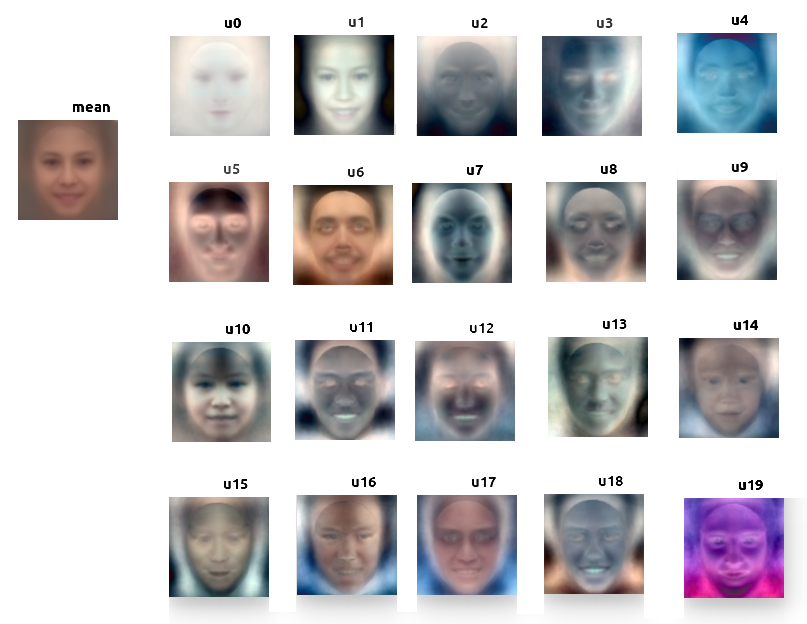
\includegraphics[width=0.5\textwidth]{results/eigenfaces3.png}
	\caption{Eigenfaces: среднее лицо и первые 20 главных компонент}
	\label{fig:eigenfaces}
\end{figure}

Авторы статьи предлагают менять освещение на усреднённом изображении именно таким образом. Ограничив матрицу собственных векторов $ V_j $ до четырёх столбцов, подбираются коэффициенты alpha, приближающие исходное изображение:
$$
\min_{\alpha} || I - \alpha V^T_j || ^2,
$$

где $ I $ --- исходное изображение. Таким образом получаются <<переосвещённые>> средние
 $ A_j^I = \alpha V_j^T $.

Когда изображения внутри кластеров выровнены, требуется найти соответствие (оптический поток) между кластерами. Проблема, однако, заключается в том, что каждый кластер содержит изображения с различным освещением, что можно выразить как различные матрицы $ V_i $ и $ V_j $ для кластеров $ i $ и $j$. Авторы предлагают для поиска плотного оптического потока между кластерами $i$ и $j$ следующую процедуру:

\begin{enumerate}
    \item Пусть $K$ --- число изображений в объединении кластеров $i$ и $j$
    \item Для каждого изображения $ I_k $ из этого объединения пользуясь матрицами $ V_i $ и $ V_j $ вычислить соответственно $ A_i^k $ и $  A_j^k $
    \item Получить два k-канальных изображения $ \textbf{A}_i = \lbrace A_i^k\rbrace_{k=1}^K $, аналогично $ \textbf{A}_j = \lbrace A_j^k \rbrace_{k=1}^K $
    \item Пользуясь сторонним алгоритмом вычислить оптический поток между $ \textbf{A}_i $ и $ \textbf{A}_j$
\end{enumerate}

В результате такого подхода соответствующие каналы двух многоканальных изображений имеют одинаковую освещённость, что нивелирует влияние освещённости на вычисление оптического потока.

В качестве стороннего алгоритма для вычисления оптического потока подойдёт любой алгоритм, способный работать с многоканальными изображениями, например SIFT flow \cite{sift_flow} или SimpleFlow \cite{simple_flow}, которому может работать с изображениями из пикселей любого вида, если для них задана функция дистанции.

Наконец, имитация старения для входного изображения $I$, текущего возраста $s$ и целевого возраста $t$ происходит следующим образом:
\begin{enumerate}
    \item Выровнять изображение $I$ c помощью конвеера из Faces Reconstruction in the Wild \cite{face_wild}
    \item Имитация текстурных изменений
    \begin{enumerate}
        \item Получить <<переосвещённые>> средние $ A^I_s $ и $ A^I_t $
        \item Вычислить оптический поток $ F_{source-input} $ между $ A^I_s $ и $I$, \\
         искривить (warp) $  A^I_s  $ c помощью этого потока, получив $ J_s $
        \item Вычислить оптический поток $ F_{target-input} $ между $ A^I_t $ и $I$, \\
         искривить (warp) $ A^I_t   $ c помощью этого потока, получив $ J_t $
        \item Прибавить к изображению I текстурную разницу: \\
        \mbox{$ I' = I + J_t - J_s $}
    \end{enumerate}

    \item Имитация изменений в потоке
    \begin{enumerate}
        \item Пусть $ F_{target-source} $ --- оптический поток между кластерами s и t, вычисленный заранее
        \item Искривить $I'$ с помощью потока $F_{target-source}$
    \end{enumerate}

    \item Скорректировать пропорции лица: растянуть изображение так, чтобы отношение расстояния между глаз к расстоянию между глазами и ртом соответствовало среднему отношению на кластере $t$
\end{enumerate}

\begin{figure}[t]
\centering
	\begin{subfigure}[t]{0.2\textwidth}
		
\includegraphics[width=\textwidth]{ilaware_cover1.png}
		\caption{3 года \\ (оригинал)} 
	\end{subfigure}
	\begin{subfigure}[t]{0.2\textwidth}
		
\includegraphics[width=\textwidth]{ilaware_cover2.png}
		\caption{5-7}
	\end{subfigure}
	\begin{subfigure}[t]{0.2\textwidth}
		
\includegraphics[width=\textwidth]{ilaware_cover3.png}
		\caption{14-16}
	\end{subfigure}
	\begin{subfigure}[t]{0.2\textwidth}
		
\includegraphics[width=\textwidth]{ilaware_cover4.png}
		\caption{26-35}
	\end{subfigure}
	\begin{subfigure}[t]{0.2\textwidth}
		
\includegraphics[width=\textwidth]{ilaware_cover5.png}
		\caption{46-57}
	\end{subfigure}
	\begin{subfigure}[t]{0.2\textwidth}
		
\includegraphics[width=\textwidth]{ilaware_cover6.png}
		\caption{58-68}
	\end{subfigure}		
	\begin{subfigure}[t]{0.2\textwidth}
		
\includegraphics[width=\textwidth]{ilaware_cover7.png}
		\caption{81-100}
	\end{subfigure}
	\caption{Последовательная имитация взросления с использованием Illumination-aware age progression}
	\label{fig:ilaware}
\end{figure}

Результат работы алгоритма приведён на рис. \ref{fig:ilaware}.

Свой алгоритм авторы решили проверить с помощью Amazon Mechanical Turk --- сервиса, который предоставляет труд людей для решения задач, которые компьютеры пока решить не в состоянии. Они давали пользователям три изображения одного и того же человека: фото человека в исходном возрасте, реальное фото человека в целевом возрасте, синтезированное фото в целевом возрасте. Пользователю требовалось определить, какое фото в целевом возрасте является настоящим, были также варианты <<оба фото настоящие>> и <<оба синтезированные>>. Оказалось, что в 37\% случаев пользователи выбирали синтезированное фото, в 41\% --- настоящее. Результат удивил авторов настолько, что они решили оценить, насколько хорошо человек способен сравнивать лица разного возраста. В ещё одном эксперименте пользователям давали две настоящие фотографии одного и того же человека с разницей минимум в пять лет и спрашивали, один ли и тот же человек изображён на фотографиях. По результатам эксперимента оказалось, что люди значительно лучше узнают взрослых спустя разное кол-во лет, чем позврослевших детей. Так, люди узнают детей от 0 до 7 лет с разницей в 10 лет с вероятностью 57\%, с разницей в 20 лет с вероятностью 52\% и с разницей в 50 и более лет с вероятностью 33\%, то есть даже хуже, чем если бы люди бросали монетку. Данное исследование говорит о том, что возможности человека по оценке алгоритмов имитации возраста очень ограничены, и человеческая оценка не всегда может служить объективным показателем качества работы такого рода алгоритмов.

Данная статья широко освещалась в крупных СМИ \cite{wired_age} \cite{telegraph_age} \cite{today_age}. Журналисты подчёркивали реалистичность результатов, сравнивая настоящие изображения человека в целевом возрасте с синтезированными.

\newpage

\section{Структура системы автоматической имитации возраста}

\subsection{Описание конвеера имитации возраста}

Любая система имитации возраста состоит из двух компонентов:
\begin{enumerate}
\item Получение текущего возраста фото
\item Синтез нового лица по следующим данным: фото, текущий возраст, изменённый возраст
\end{enumerate}
Текущий возраст фото может быть как задан пользователем, так и получен с помощью одного из алгоритмов оценки возраста.
Во втором случае на вход алгоритму поступает изображение, а на выходе получается одно число: либо конкретный возраст (если оценка возраста решает задачу регрессии), либо возрастная группа (если решается задача классификации).

В качестве алгоритма оценки возраста в конвеере используется алгоритм CNN Age Classification \cite{cnn_age_gender}, описанный ранее в разделе <<Автоматическое определение возраста>>. Данный алгоритм принимает на вход изображение лица, масштабирует его до размеров, совпадающих с размером входного слоя нейросети, затем выполняет прямой проход по нейросети и получает значения на нескольких выходах нейросети, по одному на каждый возрастной кластер. Результирующим кластером считается тот, который имеет наибольшее значение на своём выходе.
Код, загружающий изображение в нейросеть, написан на Python, проход по нейросети выполняется с помощью фреймворка Caffe. Изображение передаётся через файл, скрипту на Python передаётся имя файла. Номер результирующего кластера выдаётся в стандартный вывод.

Второй компонент конвеера, синтезирующий лица, построим на основе техник, описанных в статье Illumination-Aware Age Progression. Данный алгоритм взят за основу как наиболее актуальный из рассмотренных ранее. Кроме того, данный алгоритм, в отличие от Gandhi, полностью автоматический.

Общая схема работы этого алгоритма выглядит так:
\begin{enumerate}
\item Получение фото
\item Выравнивание фото
\item Имитация текстурных изменений
\item Имитация изменений в оптическом потоке
\item Коррекция пропорций лица
\end{enumerate}

Этап выравнивания фото будет подробно описан далее.

Имитация текстурных изменений включает в себя:
\begin{enumerate}
  \item Вычисление <<переосвещённых>> (relightable) средниx $ A^I_s $ и $ A^I_t $ для целевого и текущего кластеров
  \item Вычисление оптического потока $ F_{source-input} $ от $ A^I_s $ к $I$, \\
   $ J_s $ - искривление (warping) $ A^I_s $ c помощью этого потока
  \item Вычисление оптического потока $ F_{target-input} $ от $ A^I_t $ к $I$, \\
  $ J_t $ - искривление (warping) $ A^I_t $ c помощью этого потока
  \item Наложение на исходное изображение I текстурной разницы: \\
   $ I' = J_t - J_s $
\end{enumerate}

Имитация изменений в оптическом потоке по сути является преобразованием $I'$ с помощью потока $F_{target-source}$.
Коррекция пропорций лица осуществляется путём растягивания (интерполяции) изображения с исходного размера до нового, с исправленными пропорциями.

\subsection{Описание конвеера обучения}

Перед тем, как можно будет приступать к имитации возраста, необходимо вычислить оптические потоки $F_{target-source}$ для всех возможных пар $(target, source)$, на каждом $i$-м кластере получить $ V_i $ для вычисления relightable-изображений и вычислить средние пропорции лица.

Чтобы сделать это, необходимо обучающую выборку изображений также пропустить через конвейер. Структура этого конвеера следующая:
\begin{enumerate}
  \item Разбиение изображений на фиксированные кластеры по возрасту
  \item Выравнивание изображений внутри кластера
  \item Вычисление матриц $ V_i $ для каждого i-го кластера на основе выровненных изображений методом главных компонент
  \item Для каждой пары кластеров $ (A_i, A_j) $ таких, что $ i < j $:
  \begin{enumerate}
    \item для каждого $I_k$, такого, что $ I_k \in \lbrace A_i \cap A_j \rbrace $, вычислить $ A_i^k, A_j^k $
    \item сформировать многоканальные изображения $ \bold{A}_i , \bold{A}_j $  из одноканальных $ A_i^k, A_j^k $
    \item Пользуясь многоканальным алгоритмом поиска оптического потока, найти оптический поток $F_{j-i}$
  \end{enumerate}
\end{enumerate}

\hyphenation{Simple-Flow}

Одним из подходящих алгоритмов для вычисления оптического потока на изображении с произвольным числом каналов является SimpleFlow \cite{simple_flow}. В основе метода SimpleFlow лежит очевидная идея поиска в локальной окрестности каждого пикселя наиболее похожий на него пиксель. Для разрешения неоднозначностей и для компенсации шумов делается предположение, что в окрестности данного пикселя все точки имеют почти одинаковый сдвиг. Кроме того, поиск происходит на пирамиде изображений с увеличением масштаба на каждом уровне в два раза.

Алгоритм не использует значения пикселей непосредственно, а лишь сравнивает их между собой. Следовательно, алгоритм способен работать на изображении, состоящем из пикселей любого вида, если только для каждой пары пикселей задана функция расстояния $ d(x, y) $ между ними.

\subsection{Методы выравнивания}

Цель этапа выравнивания --- получить изображения лиц, как можно более близкие к т.н. нейтральному выражению лица. Нейтральное выражение лица как правило задаётся неким фиксированным положением ключевых точек на изображении, например, установленным вручную (см. рис. \ref{fig:neutral}).

\begin{figure}[t]
	\centering
	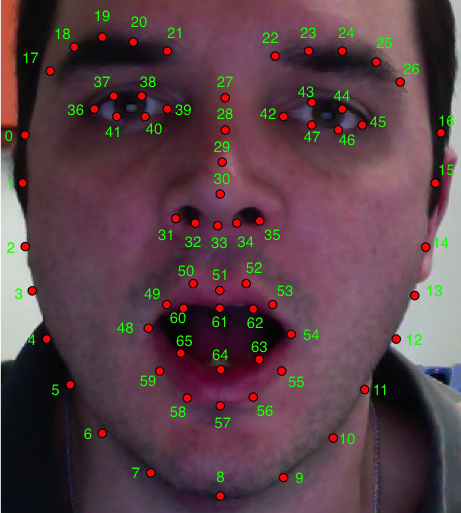
\includegraphics[width=0.3\textwidth]{avatar-annotation.png}
	\caption{Пример нейтрального расположения ключевых точек}
	\label{fig:neutral}
\end{figure}

Ещё один способ задать положение ключевых точек --- запустить один из детекторов ключевых точек на образцовой фотографии. При этом лицо на фотографии не должно выражать никаких эмоций, должно быть расположено строго анфас и ровно освещено (это желательно для работы детектора ключевых точек). Достоинство такого подхода --- во взаимозаменяемости детекторов. Недостатки --- в том, что положение точек привязывается к конкретному лицу и в том, что при детектировании ключевых точек ошибка может быть весьма серьёзной. Тем не менее данный подход используется в статье Frontalization \cite{frontalization}, а вместо фотографии используется сгенерированное (rendered) изображение 3d-модели, для целей, указанных в статье, этого вполне достаточно.

Один из способов сравнить между собой различные способы выравнивания --- определить на каждом выровненном изображении новые координаты ключевых точек и сравнивать эти координаты между собой. Однако, такой объём работы подразумевает полную переразметку всей базы тестовых изображений. В то же время поручить эту задачу детектору ключевых точек означало бы внести в измерения дополнительную ошибку, связанную с точностью детектора.

Однако, цель выравнивания изображения состоит, очевидно, в том, чтобы определённые черты лица находились в строго определённых позициях на изображении. Следовательно, если для всех выровненных изображений вычислить среднее, то при корректном выравнивании мы получим изображение лица, размытое внутри отдельных его черт, однако, с чёткими границами между чертами лица.

Для того, чтобы оценить степень размытости, введём метрику средней магнитуды: будем измерять градиент среднего изображения. Для каждого канала вычислим градиенты с помощью алгоритма Собеля, и посчитаем средний модуль градиентов по всем каналам.

Далее описаны методы выравнивания, которые были реализованы и протестированы в ходе проведения данной работы.

\subsubsection{Collection flow}

Авторы статьи Illumination-aware Age Progression \cite{illumination_aware} выполняют входное выравнивание с помощью собственного алгоритма Collection flow \cite{collection_flow}.
 
Данный алгоритм вычисляет плотный оптический поток между парами лиц на заданной коллекции изображений лиц.
Для этого для каждого изображения из коллекции делается следующее:

\begin{enumerate}
  \item Изображение проецируется на подпространство низкой размерности с целью получить нейтральное выражение лица
  \item От исходного изображения к проекции вычисляется оптический поток
\end{enumerate}

Затем исходят из предположения о нулевом оптическом потоке между нейтральными выражениями лица и для каждой пары изображений объединяют оптические потоки: сначала поток от исходного изображения к нейтральному, затем обратный поток от конечного изображения к нейтральному.

Алгоритм использует некоторые наблюдения за подходом Eigenfaces, в котором производится анализ коллекции изображений лиц методом главных компонент. Авторы исходят из предположения, что несколько первых главных компонент кодируют изменения в яркости отдельных черт лица, а также глобальные условия освещения. В то же время главные компоненты с меньшими собственными числами кодируют изменения в выражении и форме лица.

Это происходит из-за того, что так называемое non-rigid face motion, т.е. изменение выражения лица, состоит из следующих изменений изображения:

\begin{enumerate}
  \item Изменения в оптическом потоке (проявляются только на границах частей лица)
  \item Изменение формы частей лица, т.е. изменение нормалей (проявляются только на выпуклостях и впадинах)
  \item Изменения, связанные с заслонением одних частей лица другими (в виде анфас это только рот и глаза)
\end{enumerate}

Как видим, все эти изменения крайне разреженные, т.е. они касаются лишь отдельных небольших областей на лице. В то же время изменение освещённости (например, яркость, цвет или положение источника освещения) затрагивает практически всё лицо. А поскольку проекция лица rank-4, т.е. на подпространство из 4 главных компонент сохраняет до 90\% вариаций, то в основном в первых главных компонентах оказываются изменения изображения, связанные с освещением, если только исходная коллекция лиц была богата на различные режимы освещения.

Если эти предположения справедливы, то проецирование на подпространство из первых нескольких собственных векторов должно удалять с лица все различия в выражении. Однако, на практике такая низкоранговая проекция (low-rank projection) размывает лицо, на нём теряются мелкие детали, что дольно плохо для optical flow, поскольку алгоритму становится сложнее сравнивать между собой локальные окрестности точек.

Чтобы устранить данный эффект, для каждого изображения запускается итерационный алгоритм:
\begin{enumerate}
  \item Устанавливаем число главных компонент $ k = 4 $, для каждого изображения $ i $ инициализируем оптический поток $ F_i $ нулями (тождественное преобразование), помещаем в матрицу M все изображения $ I_i $
  \item Вычисляем проекции $ I_i' $ из матрицы $M$ c использованием первых $k$ главных компонент
  \item Вычисляем оптический поток $ F_i' $ от $I_i$ до $I_i'$, добавляем его к $ F_i $
  \item Искривляем $ I_i $ с использованием потока $ F_i' $
  \item $ k := k + 1 $
  \item Если норма L2 разности потоков $ F_i $ на текущей итерации и на предыдущей больше, чем фиксированный порог (в статье указан порог 20), то переходим к шагу 2, иначе останавливаемся
\end{enumerate}

Такой подход вычисления оптического потока по утверждению авторов хорошо справляется с различиями в освещении, альбедо, условиях съёмки, баланса белого и т.д., и в то же время приводит выражения лиц к нейтральному виду.

Кроме того, он позволяет вычислить оптический поток для всех изображений в коллекции за время $ O(n) $, а не за время $ O(n^2) $, как это было бы при попарном вычислении оптического потока.

\subsubsection{Фронтализация} 

В статье Effective Face Frontalization in Unconstrained Images \cite{frontalization} предлагается новый подход к генерации изображения с исправленным ракурсом. Авторы используют детектор ключевых точек, чтобы найти ключевые точки на входном изображении и сопоставить их с ключевыми точками на изображении образцового лица, для которого известна его точная 3d-модель. Используя эти данные, ищется поза лица в пространстве, после чего трёхмерная модель вписывается в изображение лица и генерируется изображение головы во фронтальной позе. Для восстановления частей изображения, заслонённых из-за поворота головы (например, одна из сторон носа), используется зеркально симметричная копия изображения (см. рис. \ref{fig:frontal2}).

В подробностях алгоритм выглядит следующим образом:
\begin{enumerate}
\item Пусть задано образцовое лицо, а именно:
\begin{itemize}
	\item Изображение $ I_R $, являющееся проекцией трёхмерной модели нейтрального лица
	\item Массив точек $ P = \{ P_i = (X_i, Y_i, Z_i)^T \}_{i=1}^N $ модели, проецирующихся в пиксели  $ p'_i = (x'_i, y'_i)^T  $ для всех пикселей изображения $ I_R $
	\item Массив ключевых точек $ K = \{ K_j = (X_j, Y_j, Z_j)^T \}_{j=1}^M $, проецирущихся в пиксели $ k'_j = (x'_j, y'_j)^T  $ для всех ключевых точек, найденных на изображении $ I_r $ выбранным алгоритмом поиска ключевых точек
	\item Матрица камеры $ A_R $, с помощью которой осуществлялось проецирование 3d-точек на плоскость:
	$$
	z'_i \begin{bmatrix} x'_i \\ y'_i \\ 1 \end{bmatrix}  = M_R P_i, M_R = A_R [R_R t_R],
	$$
где $ R_R $ и $ t_R $ --- соответственно матрица поворота и вектор трансляции в 3d-пространстве, $ z'_i $ --- масштабный коэффициент
\end{itemize} 
\item Найти на входном изображении $I_Q$ ключевые точки \\
$ b' = \{ b'_j = (x'_j, y'_j, 1)^T \}_{j=1}^M $ выбранным алгоритмом поиска ключевых точек
\item Найти матрицу проекции $ M_Q = A_R \left [ R_Q t_Q \right ] $ такую, что 
$$
M_Q = \argmin_{M_Q} \lbrace M_Q K - z^T b' \rbrace,
$$
где $ R_Q, t_Q $ --- соответственно матрица поворота и вектор трансляции в 3d-пространстве, $ z $ --- вектор-столбец неизвестных масштабных коэффициентов
\item С помощью матрицы $ M_Q $ спроецировать массив точек $ P $ на плоскость, получив набор 2d-точек $ p_Q $
\item Вычислить карту заслонений $ O_Q $:
\begin{enumerate}
	\item для каждого пикселя исходного изображения посчитать кол-во спроецированных туда точек из $p_Q$
	\item размыть $ O_Q $ гауссовым фильтром
\end{enumerate}
\item Создать новое изображение $ I_F $, перенести значения из пикселей $ p_Q $ изображения $I_Q$ в пиксели $p'$ изображения $I_F$
\item Проделать аналогичную операцию с $O_Q$, получив $O_F$
\item Использовать веса из $O_Q$ для заполнения заслонённых частей изображения, используюя симметрично отображённую копию $I_Q$ как источник
\end{enumerate}

\begin{figure}[t]
	\centering
	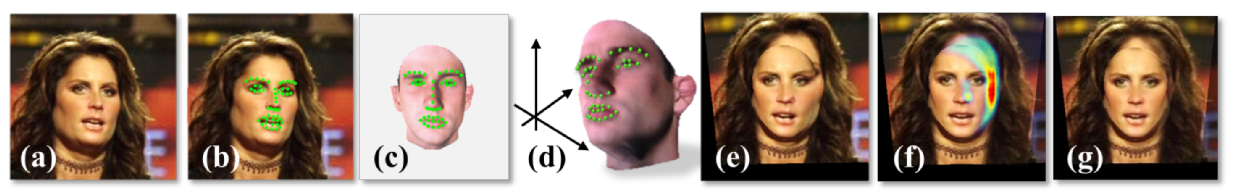
\includegraphics[width=\textwidth]{frontal2.png}
	\caption{Последовательность операций во время фронтализации}
	\label{fig:frontal2}
\end{figure}

Данный алгоритм не занимается непосредственно нейтрализацией выражения лица, однако, может быть предварять работу других алгоритмов.

\subsubsection{Искривление по ключевым точкам}

Выравнивание фото по ключевым точкам подразумевает следующую последовательность действий:
\begin{enumerate}
  \item Детектирование набора ключевых точек на лице
  \item Кадрирование лица по ключевым точкам
  \item Искривление изображения с целью выравнить позу лица
\end{enumerate}

Алгоритмы поиска ключевых точек на лице как правило основываются на двух компонентах: модель формы и модель внешнего вида. В ходе поиска ключевых точек алгоритм из начального приближения начинает итеративный поиск наилучшего расположения точек на лице, чередуя два этапа: коррекция результата с точки зрения модели формы и коррекция результата с точки зрения модели внешнего вида. Коррекция формы находит наилучшее приближение текущего расположения точек параметрами модели. Коррекция же по внешнему виду для каждой ключевой точки ищет в её окрестности наиболее подходящую по некоторым свойствам изображения в этой окрестности.

Один из первых алгоритмов поиска ключевых точек на лице --- ASM \cite{asm} --- описывал модель формы с помощью метода главных компонент, а в качестве модели внешнего вида использовал профиль яркостей пикселей вдоль нормали к контуру в каждой ключевой точке. Впоследствии на базе ASM появилось великое множество детекторов ключевых точек, отличавшихся только моделью формы. Например, один из вариантов ASM-подобного детектора ключевых точек использовал гистограммы ориентированных градиентов (HOG \cite{hog}) для описания изображения в окрестностях ключевых точек и SVM для сравнения этих дескрипторов с обученными.

Последующие алгоритмы, основываясь на похожих принципах, использовали более сложные модели формы и внешнего вида. Так, используемый в CSIRO Face Analysis SDK \cite{csiro} алгоритм за авторством Jason Saragih \cite{jsaragih} использует трёхмерную, а не двухмерную модель формы лица, основанную также на методе главных компонент. Кроме того, для поиска ключевых точек используются методы среднего сдвига (mean-shift) и свёртки с образцом. Благодаря такой технике, модельные точки буквально «прилипают» к соответствующим особенностям изображения, таким, как уголки глаз, края губ или кончик носа.

Один из популярных в последнее время методов поиска ключевых точек за авторством Zhu, Ramanan \cite{zhu_ramanan} использует дескрипторы HOG для описания локальных особенностей лица и представляет весь набор ключевых точек иерархически в виде дерева, используя технику динамического программирования для оценки весов каждого узла.

Когда положения ключевых точек найдены, требуется, сопоставив их с некими <<эталонными>> позициями, warp'ить, то есть искривить изображение так, чтобы эти ключевые точки перешли в эталонные. На первом этапе такого искривления происходит триангуляция, т.е. разбиение изображения на треугольники с вершинами в ключевых точках. Теперь для каждой точки внутри треугольника на конечном изображении мы можем, пользуясь, например, барицентрическими координатами, рассчитать соответствующую ей точку в треугольнике на исходном изображении. Однако при этом можно столкнуться с неприятным эффектом резкой границы между треугольниками, как это продемонстрировано на рисунке \ref{fig:affine}.

\begin{figure}[t]
	\centering
	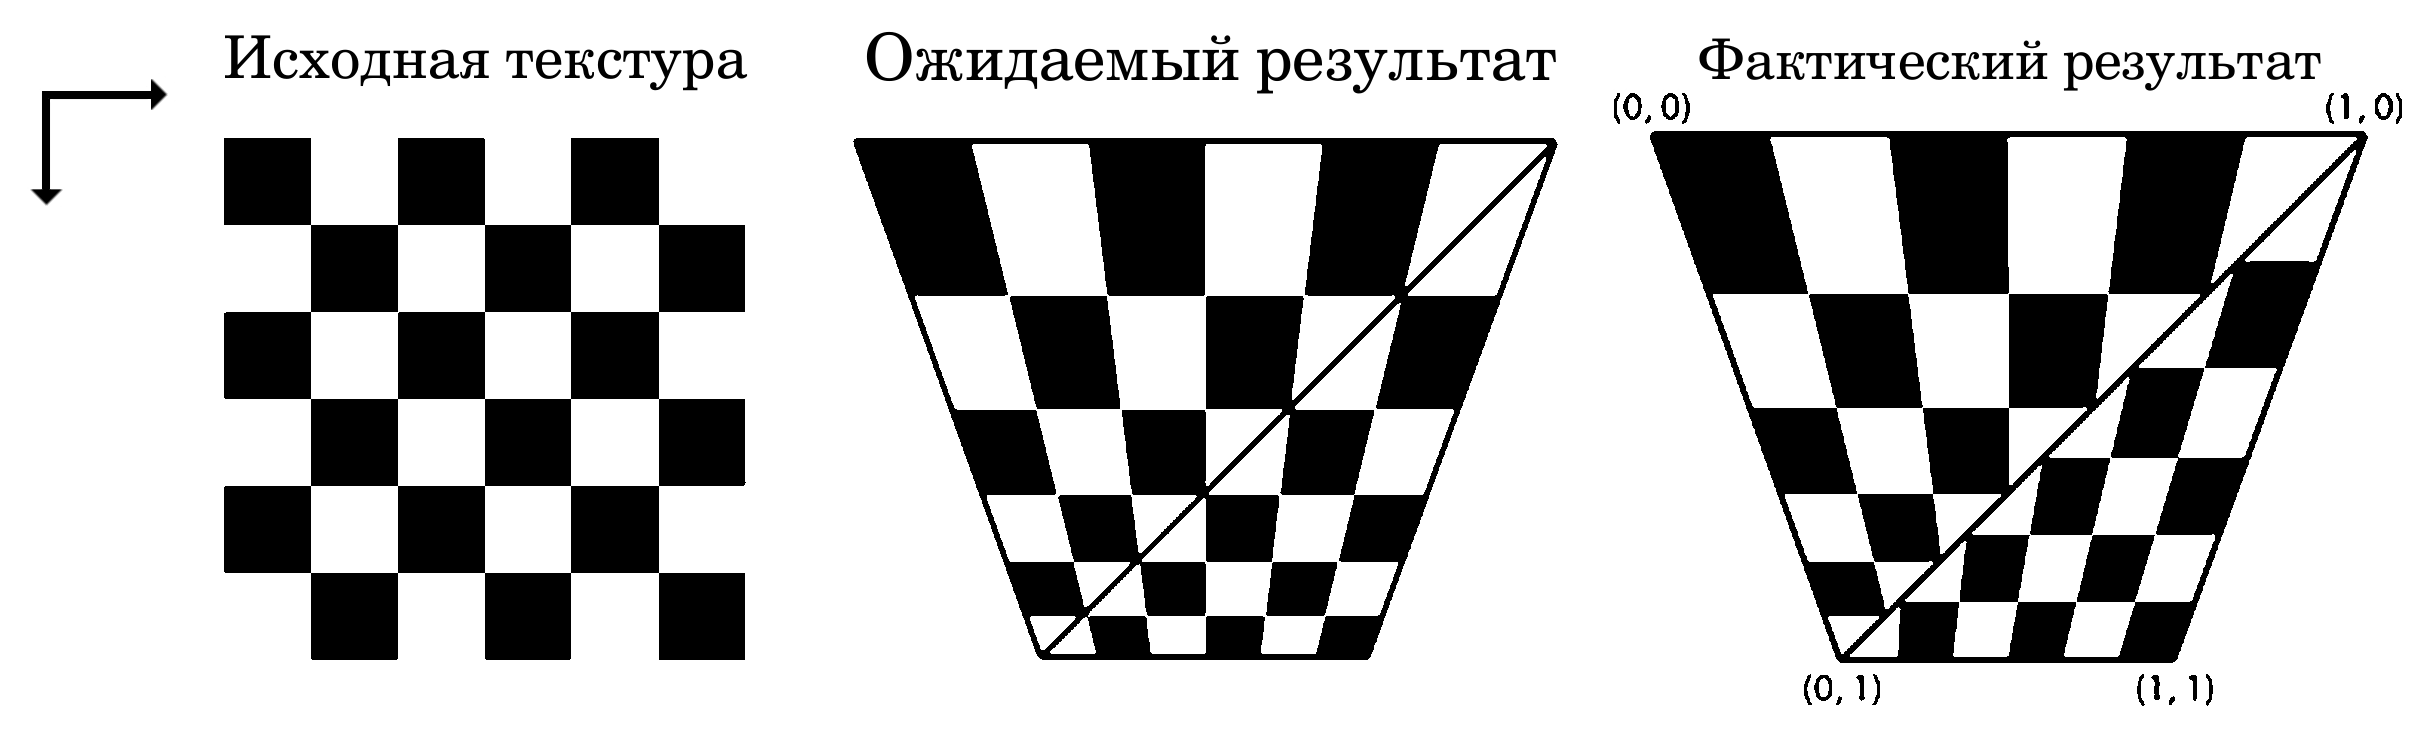
\includegraphics[width=\textwidth]{affine.png}
	\caption{Искажение изображения при кусочном афинном искривлении}
	\label{fig:affine}
\end{figure}

Для борьбы с этим эффектом используются различные техники, одна из них описывается в статье Schaefer, 2006 \cite{warping}, и именно этот подход используется в данной работе для искривления по ключевым точкам.

\subsection{Эксперименты с методами выравнивания}

В ходе реализации системы имитации возраста было решено сосредоточиться на проблеме выравнивания лица, т.е. приведения изображения лица к нейтральному виду. Дело в том, что от того, насколько точно решена эта задача, зависит то, насколько точно будут наложены текстурные изменения и изменения в оптическом потоке.

Поскольку авторы статьи Illumination-aware Age Progression прибегают к использованию собственного алгоритма Collection flow, решено было начать с него. По описанию из статьи была запрограммирована реализация на C++ с использованием библиотеки алгоритмов компьютерного зрения OpenCV. 
Алгоритм этот хоть и предназначен для вычисления оптического потока, вполне пригоден и для нейтрализации выражения лица, поскольку использует для этого промежуточное искривление исходного лица до его проекции.

Для экспериментов был взят тот же самый набор изображений лиц Adience \cite{adience}, содержащий 3210 лиц людей разного пола и возраста (на иллюстрациях <<all>>). Дополнительно были отобраны 309 фотографий одного и того же человека для проверки алгоритма в условиях, описанных в статье: когда задана большая выборка фотографий одного и того же человека (на иллюстрациях <<id>>).

Первоначально на вход алгоритму подавались фотографии, кадрированные до прямоугольника, содержащего лицо безо всякой другой предобработки. Первые результаты (см. рис. \ref{fig:exp_no}) показали, что предобработка, а именно какой-то дополнительный метод выравнивания лица, необходима: среднее изображение после работы collection flow оказалось неотличимо от среднего изображения до работы collection flow.

\begin{figure}[t]
\centering
	\begin{subfigure}[t]{0.3\textwidth}
		
\includegraphics[width=\textwidth]{results/all_no_mean.png}
		\caption{all, 15.606}
	\end{subfigure}
	\begin{subfigure}[t]{0.3\textwidth}
		
\includegraphics[width=\textwidth]{results/id2_no_mean.png}
		\caption{id, 21.1797}
	\end{subfigure}
	\caption{Collection flow: средние магнитуды для средних изображений по all и id}
	\label{fig:exp_no}
\end{figure}


Было решено добавить этап фронтализации перед вызовом collection flow. Основываясь на оригинальной Matlab-реализации, была создана собственная реализация данного подхода на С++ и OpenCV. В процессе разработки выяснилось, что алгоритм фронтализации был адаптирован для изображений в низком разрешении, в результате на изображениях большого разрешения оставались характерные артефакты в виде сетки (см. рис. \ref{fig:exp_err}). Решено было исправить эту проблему, во-первых, за счёт интерполяции точек в модели с разрешения $320 \times 320$ до $640 \times 640$, во-вторых, за счёт использования дилатации.

\begin{figure}[t]
\centering
	\begin{subfigure}[t]{0.3\textwidth}
		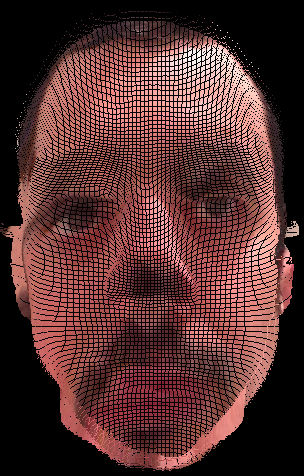
\includegraphics[width=\textwidth]{bad_model_reprojection.png}
		\caption{до дилатации}
	\end{subfigure}
	\begin{subfigure}[t]{0.3\textwidth}
		
\includegraphics[width=\textwidth]{bad_model_dilatation.png}
		\caption{после дилатации}
	\end{subfigure}
	\begin{subfigure}[t]{0.3\textwidth}
		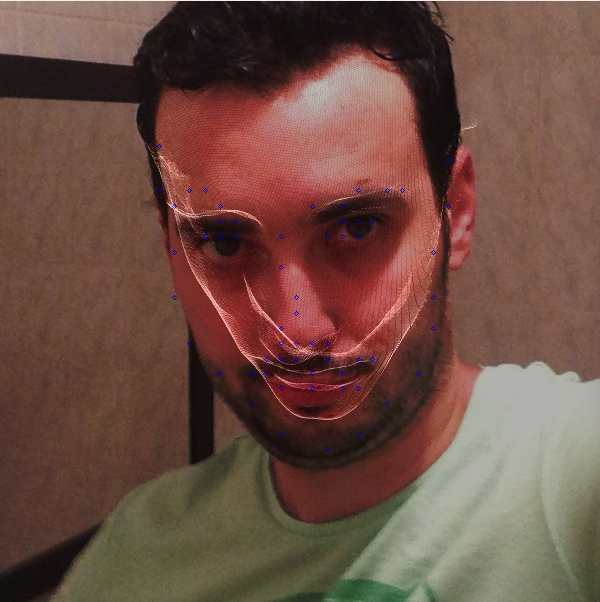
\includegraphics[width=\textwidth]{bad_model_fitting.png}
		\caption{неверная поза модели}
	\end{subfigure}
	\caption{Ошибки фронтализации}
	\label{fig:exp_err}
\end{figure}

В качестве детектора точек использовался детектор от Jason Saragin, реализованный в CSIRO Face Analysis SDK.

Также выяснилась ещё одна проблема: детектор ключевых точек от Jason Saragih плохо приспособлен к работе с неподвижными изображениями, основное его предназначение --- работа с живым видео, когда детектор улучшает свой результат от кадра к кадру. Из-за неточного соответствия ключевых точек особенностям лица поза для трёхмерной модели была найдена неправильно, в результате <<фронтализованное>> лицо теряло свои черты и искажалось (см. рис. \ref{fig:exp_err}), из-за чего точность выравнивания снижалась (см. рис. \ref{fig:exp_js}).

\begin{figure}[b]
\centering
	\begin{subfigure}[t]{0.3\textwidth}
		
\includegraphics[width=\textwidth]{results/all_myfront_mean.png}
		\caption{all, 35.9171}
	\end{subfigure}
	\begin{subfigure}[t]{0.3\textwidth}
		
\includegraphics[width=\textwidth]{results/id2_myfront_mean.png}
		\caption{id, 50.6863}
	\end{subfigure}
	\caption{Фронтализация с детектором Jason Saragih: средние магнитуды для средних изображений по all и id}
	\label{fig:exp_js}
\end{figure}

\begin{figure}[h]
\centering
	\begin{subfigure}[t]{0.3\textwidth}
		
\includegraphics[width=\textwidth]{results/all_front_mean.png}
		\caption{all, 17.6375}
	\end{subfigure}
	\begin{subfigure}[t]{0.3\textwidth}
		
\includegraphics[width=\textwidth]{results/id2_front_mean.png}
		\caption{id, 30.9887}
	\end{subfigure}
	\caption{Фронтализация с детектором Zhu Ramanan: средние магнитуды для средних изображений по all и id}
	\label{fig:exp_zr}
\end{figure}

\begin{figure}[h]
\centering
	\begin{subfigure}[t]{0.3\textwidth}
		
\includegraphics[width=\textwidth]{results/all_warped_mean.png}
		\caption{all, 20.8787}
	\end{subfigure}
	\begin{subfigure}[t]{0.3\textwidth}
		
\includegraphics[width=\textwidth]{results/id2_warped_mean.png}
		\caption{id, 27.0529}
	\end{subfigure}
	\caption{Искривление по ключевым точкам: средние магнитуды для средних изображений по all и id}
	\label{fig:exp_warp}
\end{figure}

Следующей модификацией решено было, как и в оригинальной реализации, использовать из трёхмерной модели не только голову, но и фон, чтобы избавиться от дополнительных артефактов на границе лица. Кроме того, был использован детектор ключевых точек за авторством Zhu, Ramanan.

Средние изображения демонстрируют очень точное совпадение черт лица (см. рис. \ref{fig:exp_zr}), даже несмотря на то, что никакого специального выравнивания по чертам лица не проводилось. Более того, хотя детектор Zhu, Ramanan в силу особенностей HOG ограничен точностью в 8 пикселей, это не помешало ему справиться со своей задачей лучше, чем детектор от Jason Saragih, не имеющий такого ограничения в точности.

Следующий эксперимент состоял в использовании искривления по ключевым точкам для повышения точности. Для детектирования использовался детектор Zhu, Ramanan, показавший свою более высокую точность.

Данный метод не оправдал надежд, возложенных на него: пропорции лица существенным образом искажены (см. рис. \ref{fig:exp_warp}), что особенно заметно на среднем изображении для единственного человека.

Таким образом, из всех перечисленных методов выравнивания лица наибольшую эффективность показал метод фронтализации, выполненный по оригинальной схеме с детектором Zhu, Ramanan. Также оказалось, что метрика среднего градиента плохо описывает качество работы методов выравнивания: на изображениях с детектора Jason Saragin эта метрика из-за артефактов по краям была слишком большой; в то же время метрика не смогла показать, что искривление по ключевым точкам ухудшает результат, искажая пропорции лица.

Что до collection flow, то ни одна из описанных выше техник не позволила методу улучшить результат по сравнению со входными данными. В лучшем случае на выходе collection flow выдаёт неотличимое от входного среднее, в худшем --- портит результат, размывая изображения, что показывает низкую эффективность данного метода в решении задачи выравнивания лица.

\newpage
\anonsection{Заключение}

Подводя итоги работы, нужно отметить, что в ходе её выполнения было сделано следующее:

\begin{itemize}
\item Исследованы популярные алгоритмы детектирования возраста по фотографии
\item Проведены эксперименты и собрана статистика по одному из них
\item Исследованы популярные алгоритмы имитации возраста на фотографии
\item Наиболее популярный из них изучен, определено, какие компоненты должны его составлять и с помощью каких алгоритмов должны быть реализованы
\item Реализованы наиболее важные из компонентов этого алгоритма; проведена серия экспериментов, по которой была дана оценка различным алгоритмам на роль этих компонентов
\end{itemize}

Таким образом, все цели данной работы были выполнены.

Сосредоточившись на описанных в статье алгоритмах можно подробнее изучить остальные компоненты <<конвейера>>, найти на их роль наиболее подходящие алгоритмы и оценить качество их работы.

А поскольку проблемы детектирования возраста и его имитации ещё очень далеки от своего окончательного решения, темы и задачи для будущих исследований в этих сферах закончатся ещё не скоро. 

\newpage
\phantomsection
\addcontentsline{toc}{section}{\refname}

\makeatletter\renewcommand{\@biblabel}[1]{#1.}\makeatother

\bibliographystyle{utf8gost705u}
\bibliography{bibliography}



\end{document}
